
%(BEGIN_QUESTION)
% Copyright 2006, Tony R. Kuphaldt, released under the Creative Commons Attribution License (v 1.0)
% This means you may do almost anything with this work of mine, so long as you give me proper credit

Måling av oksygeninnhold i avgassen fra en forbrenningsovn (eller kjele) er svært viktig både for maksimal brenselseffektivitet og for å minimere forurensning (spesielt dannelse av NO$_{x}$-molekyler). Ideelt vil en brenners avgass inneholde null oksygen, fordi alt oksygenet er brukt opp i forbrenningen med perfekt støkiometrisk blanding av brensel og luft. I praksis vil avgassen fra en effektivt regulert brenner ligge nær 2\%, i stedet for de vanlige 21\% i omgivelsesluft.

En måte å måle oksygeninnholdet i varm avgass på, er å bruke en {\it høytemperatur zirkoniumoksid}-detektor. Denne detektoren består av en "sandwich" av platinaelektroder på hver side av en fast zirkoniumoksid-elektrolytt. Den ene siden av denne elektrokjemiske cellen eksponeres for avgassen (prosess), mens den andre siden eksponeres for oppvarmet luft som fungerer som referanse:

$$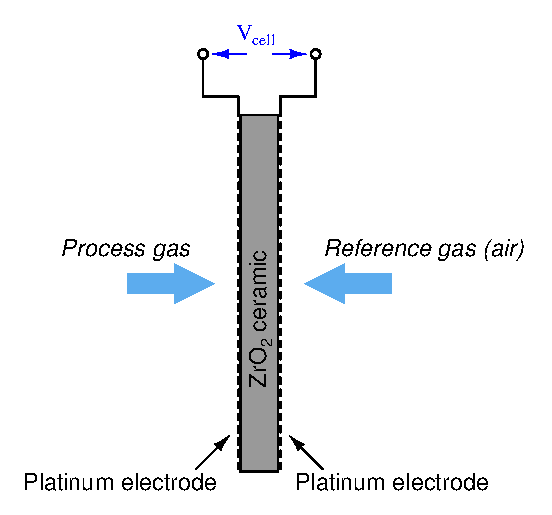
\includegraphics[width=15.5cm]{i00655x01.eps}$$

Spenningen fra cellen forutsies av Nernst-ligningen:

$$V = {{R T} \over {nF}} \ln \left({C_1 \over C_2}\right)$$

\noindent
Der,

$V$ = Spenning produsert over membranen pga. ionebytte, i volt (V)

$R$ = Universell gasskonstant (8.315 J/mol$\cdot$K)

$T$ = Absolutt temperatur, i Kelvin (K)

$n$ = Antall elektroner overført per utvekslet ion (enhetsløs)

$F$ = Faraday-konstant, i coulomb per mol (96,485 C/mol e$^{-}$)

$C_1$ = Konsentrasjon i målt løsning, i mol per liter løsning ($M$)

$C_2$ = Konsentrasjon i referanseløsning (på motsatt side av membranen), i mol per liter løsning ($M$)

\vskip 10pt

For at cellen skal fungere korrekt må den holdes ved høy temperatur (omtrent 800$^{o}$ C). Nøyaktig måling og/eller regulering av celletemperatur er avgjørende for nøyaktig oksygenmåling.

\vskip 10pt

Forklar hvorfor temperatur er en så kritisk faktor for denne sensorteknologien, og karakteriser også forholdet mellom målt oksygeninnhold og cellespenning (altså om spenningen er direkte eller omvendt relatert til oksygeninnhold).

\underbar{file i00655no}
%(END_QUESTION)





%(BEGIN_ANSWER)

At temperatur er kritisk burde være tydelig ved å se på Nernst-ligningen. Når det gjelder oksygen/spenningsforholdet kan vi si dette: celleutgangen blir null (0) hvis prosessgassen inneholder like mye oksygen som referansen (luft).

%(END_ANSWER)





%(BEGIN_NOTES)


%INDEX% Kjemi, elektro-: Nernst-ligning
%INDEX% Måling, analytisk: oksygen (høy temperatur)

%(END_NOTES)
